\section{Apache Hadoop}\label{sec:hadoop}

\textbf{Apache Hadoop} ist ein Open-Source-Software-Projekt, mit dessen Hilfe ermöglicht wird, Programme zur Datenverarbeitung mit großen Ressourcenbedarf auf verteilten System auszuführen. Hadoop wird von der \emph{Apache Foundation} entwickelt und bietet verschiedene Komponenten an, welche vollständig skalierbar sind, von einer einfachen Installation auf einem PC bis hin zu einer Installation über mehrere Server in einem Serverzentrum. Hadoop besteht hauptsächlich aus folgenden Kernmodulen \cite{HadoopHomePage}:

\begin{description}
	\item[Hadoop Common] Gemeinsam genutzte Kernkomponenten
	\item[Hadoop YARN] Framework zur Verteilung und Ausführung von Anwendungen und das dazugehörige Ressourcen-Management
	\item[Hadoop Distributed File System] Kurz HDFS, Verteiltes Dateisystem
	\item[Hadoop MapReduce] YARN-Basiertes System zum Verarbeiten von großen Datenmengen
\end{description}

Hadoop ermöglicht es dadurch, sehr einfach mit Anwendungen umzugehen, welche große Datenmengen verarbeiten. Da es für Hadoop nicht relevant ist, auf wie vielen Servern es läuft, kann es beliebig skaliert werden, wodurch entsprechend viele Ressourcen zur Bearbeitung und Speicherung von großen Datenmengen zur Verfügung stehen können.

\begin{figure}
	\centering
	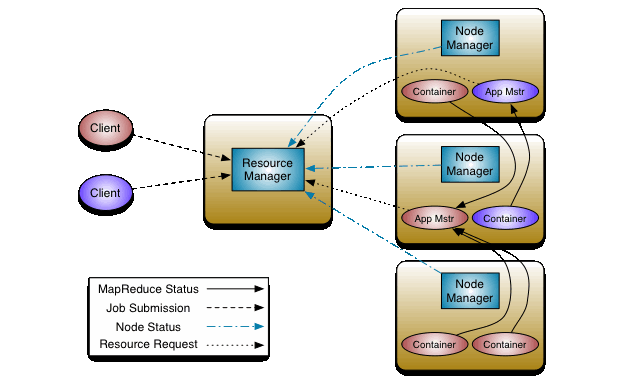
\includegraphics[width=\columnwidth]{./images/yarn_architecture.png}
	\caption[Architektur von YARN]{Architektur von YARN (entnommen aus \cite{HadoopYarnArch271})}
	\label{fig:yarnarch}
\end{figure}

Die Kernidee der Architektur von \textbf{YARN} ist die Trennung vom Ressourcenmanagement und Scheduling. Dazu besitzt der Master bzw. \emph{Controller} den \ac{RM}, welcher für das gesamte System zuständig ist und die Anwendungen im System verteilt und überwacht und somit auch als \emph{Load-Balancer} agiert. Er besteht aus zwei Kernkomponenten, dem \ac{AM} und dem \emph{Scheduler}. Der \ac{AM} ist für die Annahme und Ausführung von einzelnen Anwendungen zuständig, denen der Scheduler die dafür notwendigen Ressourcen im Cluster zuteilt.

Jeder Slave-\emph{Node} im Hadoop-Cluster besitzt einen \ac{NM}, welcher für die Überwachung der Ressourcen des Nodes und der darauf ausgeführten Anwendungs-Container zuständig ist und diese dem \ac{RM} mitteilt.

Jede YARN-Anwendung bzw. Job besteht aus einem oder mehreren Ausführungsversuchen, genannt \emph{Attempts}, denen wiederum mehrere \emph{Container} zugeordnet sind. Container können auf einem beliebigen Node ausgeführt werden und repräsentieren die Ausführung eines Tasks der Anwendung. Ein besonderer Container bildet dabei der \ac{AppMstr}, welcher innerhalb seines Attempts für das anwendungsbezogene Monitoring und die Kommunikation mit dem \ac{RM} und \ac{NM} zuständig ist und die dazu notwendigen Informationen bereit stellt \cite{HadoopYarnArch271}.

Hadoop enthält zudem einen sog. \ac{TLS}. Er ist speziell dafür entwickelt, die Metadaten und Logs der YARN-Anwendungen zu speichern und jederzeit, also auch als Anwendungshistorie, auszugeben \cite{HadoopYarnTlServer271}.

\begin{figure}
    \centering
    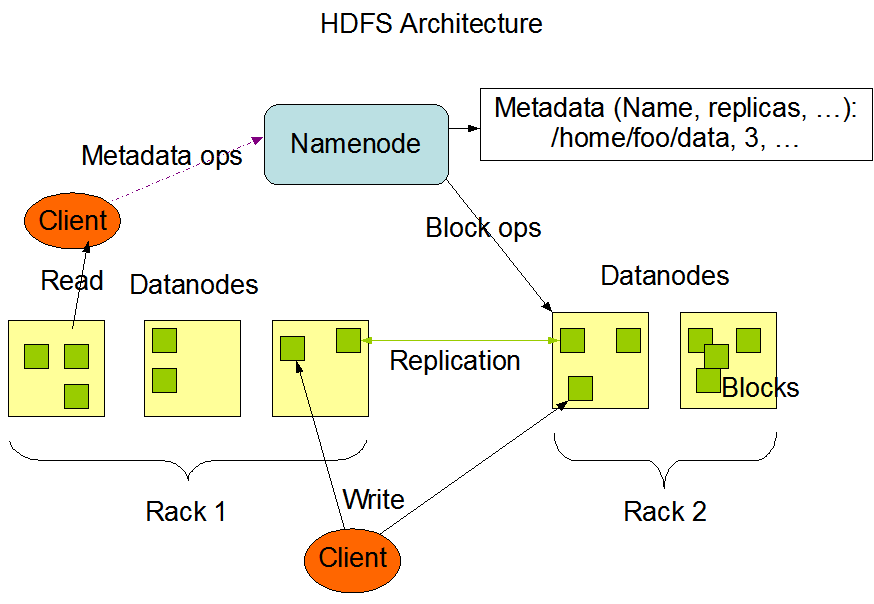
\includegraphics[width=.8\columnwidth]{./images/hdfsarchitecture.png}
    \caption[Architektur des HDFS]{Architektur des HDFS (entnommen aus \cite{HadoopHdfsDesc271})}
    \label{fig:hdfsarch}
\end{figure}

Das \textbf{HDFS} basiert auf der gleichen Architektur wie YARN und besitzt ebenfalls einen Master und mehrere Slaves, welches in der Regel die gleichen Nodes sind wie bei YARN sind. Der \emph{NameNode} ist als Master für die Verwaltung des Dateisystems zuständig und reguliert den Zugriff auf die darauf gespeicherten Daten. Die Daten selbst werden in mehrere Blöcke aufgeteilt auf den \emph{DataNodes} gespeichert. Um den Zugriff auf die Daten im Falle eines Node-Ausfalls zu gewährleisten, wird jeder Block auf anderen Nodes repliziert. Dateioperationen (wie Öffnen oder Schließen) werden direkt auf den DataNodes ausgeführt, sie sind darüber hinaus auch dafür verantwortlich, dass Clients die Daten lesen oder beschreiben können \cite{HadoopHdfsDesc271}.

\textbf{MapReduce} bietet analog zu YARN die Möglichkeit, Anwendungen mit einem großen Ressourcenbedarf, welche große Datenmengen verarbeiten, auf einem gesamten Cluster auszuführen. Dazu werden bei einem MapReduce-Job die Eingabedaten aufgeteilt, anschließend von den sog. \emph{Map Tasks} verarbeitet und deren Ausgaben von den sog. \emph{Reduce Tasks} geordnet. Für die Ein- und Ausgabe der Daten wird in der Regel das HDFS, für die Ausführung der einzelnen Tasks YARN genutzt \cite{HadoopMapRedTutorial271}. MapReduce kann auch als Vorgänger von YARN angesehen werden, da YARN auch als \emph{MapReduce Next Gen} bzw. \emph{MRv2} bezeichnet wird und aufgrund der API-Kompatibilität von YARN jede MapReduce-Anwendung in der Regel auch auf YARN ausgeführt werden kann \cite{HadoopYarnArch271,HadoopYarnOverview271}.
